\documentclass[11pt]{article}
\usepackage{polski}
\usepackage[utf8]{inputenc}
\usepackage{placeins}
\usepackage{multirow}
\usepackage{graphicx}
\usepackage{babel}
\usepackage{blindtext}
\usepackage{multicol}
\usepackage{caption}
\usepackage{textcomp}
\usepackage{siunitx}
\usepackage{minted}
\usepackage{nameref}
\usepackage{adjustbox}
\usepackage{etoolbox}
\patchcmd{\thebibliography}{\section*{\refname}}{}{}{}
\graphicspath{ {./} }
\setlength{\parindent}{20pt}

\title{\textbf{Systemy wbudowane
\\{\Large Dystrybutor napojów}}}



\author{
  {Konrad Jachimstal}\\
  \texttt{211807}
  \and
  \underline{Patryk Janicki}\\
  \texttt{211951}
  \and
  {Dobromir Kata}\\
  \texttt{176555}
}

\date{2019/2020}

\begin{document}

\maketitle
\FloatBarrier
\newpage
\tableofcontents

\newpage

\section{Wprowadzenie}
Celem zadania było stworzenie programu dla mikrokontrolera z użyciem różnych funkcjonalności (GPIO, ADC, PWM, Timer, SPI, I2C, itd.) i współpracującego z urządzeniami zewnętrznymi (wyświetlacz, akcelerometr, żyroskop, silnik, itd.). Do realizacji zadania został wybrany projekt \textbf{dystrybutora płynu} z jednym zbiornikiem na ciecz, zbudowany na podstawie mikrokontrolera \textbf{Arduino UNO R3} (Atmega 328P-AU+CH340G).

\section{Wykorzystane elementy}
\subsection{Platforma Arduino UNO R3}
\begin{itemize}
    \item mikrokontroler ATmega328P (16MHz);
    \item 32KB pamięci Flash, 2048KB SRAM;
    \item 1024B EEPROM/HEF;
    \item UART x1, SPI x2, I2C x1, PWM x6, Input Capture x1, CCP x1;
    \item Zegar 8-bit x2, zegar 16-bit x1;
\end{itemize}

\subsection{Podzespoły}
\FloatBarrier
\begin{table}[!htbp]
\begin{tabular}{|l|l|}
\hline
\multirow{6}{*}{\textbf{Urządzenia peryferyjne}} & Mini pompa wody - MY-DB5 - 5V                                           \\ \cline{2-2} 
                                                 & Ultradźwiękowy czujnik odległości JSN-SR04T \\ \cline{2-2} 
                                                 & Sonda wodoodporna z czujnikiem temperatury DS18B20                      \\ \cline{2-2} 
                                                 & Wyświetlacz LCD 2x16 z konwerterem I2C LCM1602         \\ \cline{2-2} 
                                                 & Wyświetlacz LED linijka DC-10SRWA            \\ \cline{2-2} 
                                                 & Czujnik siły nacisku RA9P - 4kg okrągły                                 \\ \cline{2-2}
                                                 & Buzzer z generatorem 5V 12mm                                 \\ \hline
\multirow{3}{*}{\textbf{Układy scalone}}         & Rejestr przesuwny 74HC595 - 8-bitowy                                    \\ \cline{2-2} 
                                                 & Tranzystor N-MOSFET IRL540NPBF                                    \\ \cline{2-2} 
                                                 & Transoptor jednokanałowy PC817                                   \\ \hline
\multirow{3}{*}{\textbf{Inne}}                   & Przycisk monostabilny, okrągły 250V/3A                            \\ \cline{2-2} 
                                                 & Dioda Schottky 1N5819 1A                                                \\ \cline{2-2} 
                                                 & Dioda LED 5mm czerwona                                                  \\ \hline
\end{tabular}
\end{table}

\section{Funkcjonalności i opis}

\subsection{Wykrywanie naczynia}
Umieszczony w podstawie czujnik ultradźwiękowy wysyła fale prostopadle do górnej części dystrybutora i odbiera echo sygnału. Efektem zakrycia czujnika jest zbyt krótki sygnał, co skutkuje zerową wartością na wyjściu. Program sprawdza, czy od ostatniego poprawnego pomiaru minął czas określony w konfiguracji ($1s$). Pomiar wykonywany jest co $100ms$.

\subsection{Sygnalizacja stanu za pomocą diody LED}
Dioda LED umieszczona nad naczyniem sygnalizuje czy naczynie zostało wykryte, zgodnie ze stanem uzyskanym przy pomocy czujnika ultradźwiękowego. W przypadku zapalenia się diody urządzenie jest gotowe do rozpoczęcia procesu nalewania.

\subsection{Miganie diody LED podczas nalewania}
Podczas trwania procesu nalewania dioda naprzemiennie otrzymuje na wyjście stan wysoki i niski, przy czym każdy z nich trwa $500ms$, sygnalizując tym samym nalewanie. 

\subsection{Pomiar poziomu cieczy w zbiorniku}
Przybliżony poziom cieczy uzyskiwany jest za pomocą czujnika nacisku umieszczonego pod zbiornikiem. Program odczytuje wartość na wejściu analogowym,przy czym rezystancja odzwierciedla siłę nacisku. Otrzymywana wartość jest skalowana z pominięciem wagi pustego zbiornika. Należy mieć jednak na uwadze,
że czynniki zewnętrzne mogą wpływać na wynik pomiaru - temperatura ($10\%$) oraz wilgotność ($20\%$). Pomiar jest wykonywany co $1s$.

\subsection{Wyświetlanie poziomu cieczy w zbiorniku}
Piny wyświetlacza 10-segmentowego w kolorze czerwonym zostały połączone z dwoma złączonymi 8-bitowymi rejestrami przesuwnymi (łącznie 16 bitów). Przetwarzana wartość została wyskalowana tak, 
aby przy pokryciu pompy wodą w zbiorniku wynosiła zero. Wartości otrzymywane z czujnika są z zakresu $0-1024$. Otrzymana wartość z zakresu $800-1024$ (z uwzględnieniem wagi zbiornika i elementów podtrzymujących) mapowana jest na $0-10$, co odpowiada liczbie segmentów 10-poziomowego wyświetlacza.

\subsection{Komunikaty dźwiękowe z użyciem buzzera}
Urządzenie zostało wyposażone w buzzer z generatorem, którego dźwięk informuje o dokonanej akcji lub stanie urządzenia. Zasilanie buzzera sterowane jest poprzez wyjście $GPIO$ z $PWM$ na mikrokontrolerze,
a poprzez odpowiednie napięcie na wyjściu ustalany jest ton, który pozwala na zróżnicowanie sygnałów dźwiękowych.\\

Sygnały dźwiękowe wydawane przez urządzenie:\\
\begin{itemize}
  \item sygnał ciągły - czas trwania:
  \begin{itemize}
      \item użycie przycisku przełączenia programu - $200ms$;
      \item użycie przycisku akcji - $1s$;
      \item samoczynne przełączenie ekranu na wyświetlaczu LCD - $100ms$;
      \item pomyślne zakończenie procesu nalewania - $500ms$;
      \item zmiana stanu - wykryte naczynie - $50ms$;
    \end{itemize}
  \item sygnał odmowy - sekwencja:
  \begin{itemize}
      \item sygnał ciągły - $200ms$;
      \item brak sygnału - $50ms$;
      \item sygnał ciągły - $500ms$;
    \end{itemize}
\end{itemize}

\subsection{Pomiar temperatury cieczy w zbiorniku}
Pomiar temperatury odbywa się za pomocą interfejsu OneWire. Pomiar i wyświetlenie wartości następuje co $20s$.
Wartość zaokrąglana jest do jednego miejsca po przecinku i wyświetlana w stopniach Celsjusza. 

\begin{itemize}
    \item dokładność pomiaru: $0.5$\textdegree{}C (w zakresie od $-10$\textdegree{}C do $85$\textdegree{}C);
    \item zakres pomiaru: od $-55$\textdegree{}C do $125$\textdegree{}C;
\end{itemize}

\subsection{Kontrola programu za pomocą przycisku}
W urządzeniu zlokalizowano dwa przyciski monostabilne. Program wykrywa naciśnięcie przycisku i wykonuje odpowiednie akcje.
Zielony przycisk służy do przełączenia ilości płynu, jaki ma zostać nalany. Dostępne wartości dotyczące ilości płynu zdefiniowane 
są w pamięci programu. Czerwony przycisk służy do rozpoczęcia procesu nalewania. Akcje wykonywane są w momencie, gdy przycisk
zostanie zwolniony - "on key up".

\subsection{Sterowanie pompą}
 
Układ elektroniczny został podzielony na dwie części: jedna jest powiązana elektrycznie ze sterownikiem i jej zadaniem jest sterowanie diodą LED w transoptorze, druga część obejmuje układ dołączony do tranzystora.

Pompa zasilana jest z zewnętrznego układu zasilania, odseparowanego galwanicznie od mikrokontrolera. Włączanie oraz wyłączanie pompy obsługiwane jest za pomocą pinu cyfrowego z $PWM$\footnote{PWM - https://enterius.eu/wsparcie/artykuly-techniczne/modulacja-pwm-co-to-jest} podającego zasilanie na transoptor, który steruje bramką / załączeniem tranzystora MOSFET odpowiedzialnego za pracę pompy. 
Ze względu na indukcyjny charakter obciążenia, równolegle do odbiornika, została dodana dioda zabezpieczjąca i chroniąca tranzystor przed zniszczeniem od napięcia samoindukcji, które obciążenie wygeneruje podczas wyłączania.


\FloatBarrier
\section{Podział obowiązków}
\begin{table}[!htbp]
\begin{tabular}{|c|c|c|c|}
\hline
                             & Konrad Jachimstal & Patryk Janicki & Dobromir Kata  \\ \hline
Dokumentacja                 & \bullet           & \bullet        & \bullet        \\ \hline
Pompa, transoptor            &                   & \bullet        & \bullet        \\ \hline
Wyświetlacze, rejestr        & \bullet           & \bullet        &                \\ \hline
Czujnik ultradźwiękowy       & \bullet           & \bullet        & \bullet        \\ \hline
Czujnik nacisku              & \bullet           & \bullet        & \bullet        \\ \hline
Czujnik temperatury          & \bullet           & \bullet        & \bullet         \\ \hline
Dioda LED                    & \bullet           & \bullet        & \bullet         \\ \hline
Przyciski                    & \bullet           & \bullet        & \bullet        \\ \hline
Sygnały dźwiękowe            &                   & \bullet        &                \\ \hline
Przewody                     & \bullet           &                & \bullet        \\ \hline\hline
\textbf{Zaangażowanie}       & $80\%$            & $90\%$         & $80\%$         \\ \hline
\end{tabular}
\end{table}

\newpage
\section{Instrukacja użytkowania}
\subsection{Schemat}

\begin{multicols}{2}
\includegraphics[scale=0.5]{schem.jpg}
1. Poziom płynu w zbiorniku (0 - 10)\\
2. Główny wyświetlacz\\
3. Przycisk zmiany programu\\
4. Przycisk akcji (nalewania)\\
5. Dioda sygnalizująca stan\\
6. Kran do dystrybucji płynu\\
7. Czujnik wykrywający naczynie
\end{multicols}


\subsection{Podłączenie}
W urządzeniu znajdują się dwa gniazda, USB oraz gniazdo DC. Aby urządzenie działało poprawnie należy zasilić oba gniazda. Po podłączeniu gniazda USB do prądu na ekranie LCD pojawi się ekran główny. 

\subsection{Wybór ilości płynu}
W celu zmiany domyślnej wartości ilości płynu ($40ml$) należy raz wcisnąć zielony przycisk $(3)$, co będzie skutkowało pojawieniem się ekranu wyboru ilości płynu na wyświetlaczu $(2)$. Aby zmienić tę wartość należy wcisnąć zielony przycisk $(3)$, co spowoduje przełączenie wartości na ekranie $(2)$. Dostępne wartości to: $40ml$, $100ml$, $150ml$, $200ml$, $250ml$, $330ml$. Aby zapisać wybraną ilość płynu należy odczekać $4s$, wtedy usłyszymy dzwięk a na ekranie głównym $(2)$ pojawi się wybrana przez nas ilość płynu.
\newpage

\subsection{Nalewanie}
Przed rozpoczęciem nalewania należy ustawić naczynie w wyznaczonym miejscu $(7)$. Poprawne ustawienie naczynia zostanie zasygnalizowane zapaleniem się diody $(5)$ oraz sygnałem dźwiękowym. Nalewanie z kranu $(6)$ rozpocznie się po naciśnięciu czerwonego przycisku $(4)$. Podczas nalewania dioda $(5)$ zacznie migać oraz na ekranie $(2)$ pojawi się odpowiadni komunikat informujący o procesie nalewania. Jeżeli podczas nalewania naczynie zostanie usunięte, proces zostanie przerwany. Zakończenie nalewania zasygnalizowane zostanie dźwiękiem, zgaśnięciem diody $(5)$ oraz odpowiednim komunikatem na ekranie głównym $(2)$. 

\subsection{Poziom płynu w zbiorniku}
Poziom płynu odzwierciedlony jest na wyświetlaczu $(1)$ znajdującym się po lewej stronie panelu przedniego urządzenia. W przypadku kiedy poziom płynu będzie niewystarczający nalewanie nie zostanie rozpoczęte a na ekranie $(2)$ pojawi się stosowny komunikat. W przypadku gdy podczas nalewania poziom płynu w zbiorniku spadnie poniżej minimum, nalewanie zostanie przerwane.

\section{Schemat układu sterowania pompą}
Podczas konstrukcji urządzenia zaszła potrzeba separacji galwanicznej dwóch bloków układu (platformy oraz pompy).\\
\begin{adjustbox}{width=320,center}
\noindent\makebox[\textwidth]{%
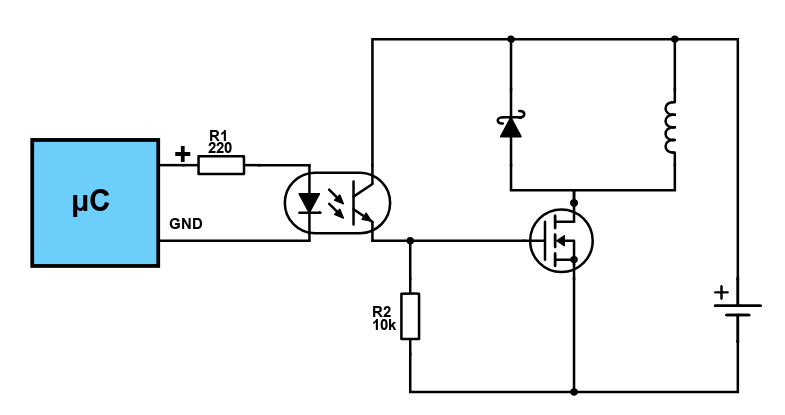
\includegraphics[scale=0.55]{uklad.png}
}
\end{adjustbox}

\section{Wykorzystane biblioteki}
\subsection{NewPing}
Biblioteka\footnote{NewPing - https://bitbucket.org/teckel12/arduino-new-ping} wykorzystywana do pomiaru odległości z wykorzystaniem czujnika ultradźwiękowego SR04T. Do pomiaru odległości wykorzystywane są dwa piny (TRIGGER i ECHO), obsługiwane w bibliotece za pomocą Port Registers\footnote{Port Registers - https://www.arduino.cc/en/Reference/PortManipulation}. W celu dokonania pomiaru na pinie TRIGGER wyzwalany jest sygnał wysoki na $10$\si\micro$s$, co powoduje wysłanie przez sensor 8 impulsów w częstotliwości $40kHz$. Detekcja ultradźwięków realizowana jest na pinie ECHO w trybie odczytu. Długość trwania stanu wysokiego na tym pinie jest proporcjonalna do odległości.

\subsection{ShiftRegister74HC595}
Biblioteka\footnote{ShiftRegister74HC595 - https://github.com/Simsso/ShiftRegister74HC595} usprawnia obsługę rejestrów przesuwnych, dodatkowo obsługuje łączenie rejestrów. W tym przypadku połączono dwa 8-bitowe rejestry przesuwne 74HC595, które pozwalają na obsługę 10 segmentów. Biblioteka wykorzystuje piny DATA (dane), CLOCK (przesunięcie) oraz LATCH (odblokowanie). W bibliotece wykorzystano funkcję shiftOut z Arduino, która zarządza przekazaną zmienną i przekazuje dane na pin DATA, sterując jednocześnie pinem CLOCK.

\subsection{LiquidCrystal\_I2C}
Biblioteka\footnote{LiquidCrystal\_I2C - https://github.com/fdebrabander/Arduino-LiquidCrystal-I2C-library} wykorzystuje interfejs I2C do komunikacji z konwerterem wyświetlacza. Komunikacja odbywa się przy użyciu biblioteki Wire, która wysyła sekewncje bitów do urządzeń na magistrali I2C. Biblioteka odwołuje się do konwertera, zlokalizowanego pod adresem $0x27$, natomiast wykorzystanie adresów wewnętrznych konwertera pozwala na wykonywanie akcji związanych z obsługą wyświetlacza.

\subsection{DS18B20}
\indent Sterowanie czujnikiem temeratury DS18B20 odbywa się za pomocą biblioteki DS18B20\footnote{DS18B20 - https://github.com/matmunk/DS18B20}, który komunikuje się za pomocą interfejsu 1-Wire (OneWire)\footnote{OneWire - https://pl.wikipedia.org/wiki/1-Wire}. Do jednej lini danych możemy podłączyć wiele urządzeń, które posiadają swój unikatowy 64-bitowy adres. Przesyłanie rozpoczyna się sekwencją bitów, wysłaniem impulsu reset (zwarciu na 480\si\micro$s$ do masy), a następnie potwierdzenie obecności przez każde urządzenie poprzez zwracie linii danych do masy na 60\si\micro$s$. Logiczna jedynka to krótki (1-15\si\micro$s$) impuls o stanie niskim, następnie stan wysoki o długości 60\si\micro$s$. Opadające zbocze impulsu aktywuje przerzutnik, który taktuje wewnętrzny mikroprocesor, co powoduje odczyt danych z lini po ok. 30\si\micro$s$ od momentu pojawienia sie zbocza narastającego. Ze względu na wewnętrzne opóźnienia urządzenia czas trwania pojedyńczego sygnału musi wynosić 60\si\micro$s$.
Po przesłaniu 8 bitów następuje wysłanie komendy (rozkazu, ośmiobitowego). Ewentualne błędy w transmisji mogą być wykryte za pomocą wbudowanego algorytmu CRC-8\footnote{CRC-8 - https://pl.wikipedia.org/wiki/Cykliczny$_$kod$_$nadmiarowy}.
Biblioteka wykorzystuje polecenia 0xF0 oraz 0x33 do wykrywania urządzeń podłączonych do magistrali OneWire.

\newpage
\section{Opis algorytmu}
Program został stworzony w podstawowym IDE dla Arduino, umieszczony w projekcie o nazwie $fluid-dispenser.ino$. W celu zwiększenia czytelności kod został podzielony na sekcje.

\subsection{Sekcje deklaracji stałych}
W tej sekcji zadeklarowano piny odpowiadające poszczególnym funkcjonalnościom (IN/OUT NUMBERS), indeksy poszczególnych zadań (TASK NAMES - więcej informacji w punkcie "\ref{zadania} \nameref{zadania}") oraz inne wartości wykorzystywane w programie (CONFIGURATION) takie jak czas detekcji naczynia, czasy wygasania ekranów oraz dostępne pojemności.
\begin{minted}{cpp}
    // =================== IN/OUT NUMBERS ==================
    // Buttons
    #define TOGGLE_BUTTON_PIN 4 // IN
    #define BUZZER_PIN 5 // OUT
    ...
    // ===================== TASK NAMES ====================
    #define MEASURE_DISTANCE_TASK 0
    #define TOGGLE_BUTTON_TASK 1
    ...
    // =================== CONFIGURATION ===================
    #define CUP_DETECTION_TIME 1000
    #define BUTTONS_DEBOUNCE_TIME 200
    ...
\end{minted}

\subsection{Sekcja deklaracji zmiennych globalnych}
Sekcja ta zapisuje dane ulegające zmianie podczas działania programu np. takie jak: czas trwania programu, ton brzmienia buzzera, czas trwania dzwięku, stan diody czy stan przycisków.  
\begin{minted}{cpp}
    // ===================== VARIABLES =====================
    // Multitasking millis variables
    unsigned long currentMillis = 0;
    unsigned long prevMillis[11];
    // Button states
    boolean toggleButtonPressed = false;
    ...
\end{minted}

\subsection{Sekcja instancji klas bibliotek}
W celu przyspieszenia pracy i zmniejszenia ilości kodu użyto zewnętrznych bibliotek przeznaczonych do obsługi wykorzystanych w urządzeniu elementów. W tej sekcji zadeklarowano instancje klas bibliotek dla:
\begin{itemize}
    \item czujnika ultradźwiękowego;
    \item rejestru przesuwnego;
    \item wyświetlacza LCD;
    \item czujnika temperatury;
\end{itemize}
\begin{minted}{cpp}
    // ===================== INSTANCES =====================
    NewPing sonar(TRIGGER_PIN, ECHO_PIN, MAX_DISTANCE);
    ShiftRegister74HC595 sr(2, SHIFTREG_SERIAL_DATA_PIN, SHIFTREG_...);
    LiquidCrystal_I2C lcd(0x27, 16, 2);
    DS18B20 ds(TEMPERATURE_SENSOR_PIN);
\end{minted}

\subsection{Sekcja inicjalizacji}
Inicjalizacja programu rozpoczyna się ustawieniem pinów na wyjście lub wejście w zależności od pełnionej funkcji. Kolejno inicjowany jest wyświetlacz oraz na jego ekranie wyświetlany jest ekran główny (informacja o temperaturze oraz wybrana pojemność). Szczegóły implementacji wyświetlania ekranów opisane zostały w sekcji \ref{ekran}.
\begin{minted}{cpp}
    // ======================= SETUP =======================
    void setup() {
      pinMode(TOGGLE_BUTTON_PIN, INPUT);
      pinMode(ACTION_BUTTON_PIN, INPUT);
      pinMode(BUZZER_PIN, OUTPUT);
      pinMode(PUMP_PIN, OUTPUT);
      pinMode(DIODE_PIN, OUTPUT);

      lcd.init();
      lcd.backlight();
      displayHomeScreen();
    }
\end{minted}

\subsection{Sekcja pętli programu}
W głównej pętli programu zapisywane jest aktualny czas od rozpoczęcia pracy. Jest on wykorzystywany do sterowania czasem poszczególnych zadań, ze względu na brak wykorzystania opóźnień ($delay$). Następnie sprawdzane są warunki zajścia poszczególnych akcji (szczegóły obsługi zadań w sekcji \ref{zadania}). Dodatkowo w pętli umieszczono również przechwytywanie stanu dźwięków oraz diod (szczegóły w sekcji \ref{zadania}).
\begin{minted}{cpp}
    // ======================= LOOP ========================
    void loop() { 
      currentMillis = millis();
    
      if (canPerformTask(MEASURE_DISTANCE_TASK, 100)) {
        performMeasureDistanceTask();
      }

      ...

    // Handle sounds
      handleSoundsTask();
    
    // Handle diodes
      handleDiodesTask();
    
    // Set pump state
      digitalWrite(PUMP_PIN, isPumpActive);
    }
\end{minted}

\subsection{Sekcja zadań}
\label{zadania}
W celu zwiększenia czytelności kodu oraz uogólnienia czasu odstępu pomiędzy zadaniami, wykorzystano tablicę \mintinline{cpp}{prevMillis[]} oraz funkcję \textcolor{blue}{\mintinline{cpp}{canPerformTask()}}. Jako indeksy tablicy użyte zostały stałe. W elementach tablicy przechowywany jest czas ostatniego wykonania zadania. Szczegóły implementacji funkcji w sekcji \ref{funkcje}.
\begin{minted}{cpp}
    // ======================= TASKS =======================
    // ----------------------- T00: Measure distance task
    void performMeasureDistanceTask() {
      int distance = sonar.ping_cm();
      if (distance > 30) return;
      ...
    }

    // ----------------------- T01: Toggle button task
    void perfomToggleButtonTask() {
      if (isPumpActive) {
        return;
      }
      ...
    }
    
    // ----------------------- T02: Action button task
    void perfomActionButtonTask() {
      if (isCupPresent() && !isVesselAlreadyFilled) {
        pumpStartTime = currentMillis;
        isPumpActive = true;
        isDiodeBlinking = true;
      }
      ...
    }
    
    // ----------------------- T03: Expire toggle task
    void performExpireToggleTask() {
      isToggleActivated = false;
      ...
    }
    
    // ----------------------- T04: Expire no vessel task
    void performExpireNoVesselTask() {
      noVesselActivated = false;
      displayHomeScreen();
      ...
    }
\end{minted}

\newpage
\subsection{Sekcja dźwięków}
\label{dzwieki}
Operacje na dźwiękach wykonywane są za pomocą podania napięcia na wyjście pinu w odpowiednich sekwencjach oraz odstępach czasowych. Manipulując napięciem uzyskujemy odpowiedni ton dzwięku wydobywający się z podłączonego buzzera zawierającego generator. W sekcji kodu zawarto zmienne pozwalające obliczyć czas, który upłynął od zmiany wartości dźwięku.
\begin{minted}{cpp}
    // ----------------------- S00: Beep
    boolean beepSoundActive = false;
    unsigned long beepSoundStartTime = 0;
    void handleBeepSound() {
      ...
      int buzzerValue = beepSoundActive ? beepTone : 0;
      analogWrite(BUZZER_PIN, buzzerValue);
    }
    
    // ----------------------- S01: Negative
    boolean negativeSoundActive = false;
    unsigned long negativeSoundStageTime = 0;
    unsigned int negativeSoundStage = 0;
    boolean negativeSoundStageSetted = false;
    void handleNegativeSound() {
      ...
    }
\end{minted}


\subsection{Sekcja ekranów}
\label{ekran}
Każdy ze stanów pracy urządzenia posiada ekran informujący użytkownika o wykonywaniu akcji lub zmianie ustawień. Dodatkowo podczas przełączania zawartości wyświetlacza ustawiane są zmienne globalne (\mintinline{cpp}{isHomeScreenActive}, \mintinline{cpp}{isDoneScreenActive}, ...), które informują o tym, który ekran jest aktualnie wyświetlony. Zmienne te pozwalają określić, czy inny ekran może zostać przełączony w danym momencie.
\begin{minted}{cpp}
    // ----------------------- SC00: Home
    void displayHomeScreen() {
      isHomeScreenActive = true;
      lcd.clear();
      lcd.print("TEMP:     " + String(temperature, 1) + "C");
      lcd.setCursor(0, 1);
      lcd.print("SELECTED: " + volumeText(VOLUMES[toggleStage]));
    }
    ...
\end{minted}

\subsection{Sekcja funkcji}
\label{funkcje}
\subsubsection{canPerformTask()}
Funkcja \textcolor{blue}{\mintinline{cpp}{canPerformTask()}} zwraca prawdę, jeśli zadanie może zostać ponownie wykonane, jednocześnie aktualizując czas wykonania zadania. Wykorzystywana jest ona przy wykonywaniu poszczególnych zadań. 
\begin{minted}{cpp}
    // Alternative for delay() function
    boolean canPerformTask(int index, unsigned long ms) {
    // Check if task will should be performed
      if (abs(currentMillis - prevMillis[index]) >= ms) {
    // Update last perform time
        updateTaskTime(index);
        return true;
      }
      return false;
    }
\end{minted} 

\subsubsection{updateTaskTime()}
Funkcja aktualizuje czas zadania o podanym indeksie.
\begin{minted}{cpp}
    // Update prev time
    void updateTaskTime(int index) {
      prevMillis[index] = currentMillis;
    }
\end{minted}

\subsubsection{isCupPresent()}
Funkcja pozwala na sprawdzenie, czy naczynie zostało wykryte. Liczba prawidłowych pomiarów czujnika ultradźwiękowego jest zliczane poprzez zmienną globalną \mintinline{cpp}{echoMeasurementsCount} w zadaniu $MEASURE\_DISTANCE\_TASK$. W przypadku gdy naczynie zostanie postawione na czujniku, oczekiwane są nieprawidłowe pomiary (brak pomiaru). Jeśli liczba prawidłowych pomiarów jest równa 0, a czas od ostatniego pomiaru jest większy od $CUP\_DETECTION\_TIME$, to wówczas uznajemy, że naczynie zostało wykryte.

\begin{minted}{cpp}
    // Check if ultrasound sensor is covered
    boolean isCupPresent() {
      return echoMeasurementsCount == 0 && 
             currentMillis - echoMeasurementTime >= CUP_DETECTION_TIME;
    }
    ...
\end{minted}

\subsection{Podsumowanie}
W powyższym przedstawieniu zostały zaprezentowane jedynie najważniejsze, elementarne fragmenty kodu, mające istotny wpływ na strukturę i działanie programu. W celu zapoznania się z całym kodem, należy zasięgnąć źródła dostępnego w repozytorium\footnote{Repozytorium - https://github.com/janicky/fluid-dispenser}.



\section{Analiza rodzajów i skutków możliwych błędów}
\FloatBarrier

\subsection{Awaria wyświetlacza znakowego i segmentowego}
Ze względu na to, że wyświetlacz jest urządzeniem końcowym i nie pobierami z niego żadnych danych, nie jesteśmy w stanie wykryć jego awarii.

\subsection{Awaria pompy}
Pompa działa jako samodzielne urządzenie przez co nie możemy wykryć jej awarii.

\subsection{Awaria czujników}
Wykorzystanie czujniki pozwalają na autodetekcję niesprawności ze względu na to, że podczas działania programu pobierane są z nich dane. Podczas gdy dane pobrane z czujnika będą wykraczały po za wartości regularne lub czujnik nie będzie wysyłał odczytów, możemy stwierdzić, że dany czujnik uległ uszkodzeniu. 

\newpage
\subsection{Awaria diody, przycisków, buzzera}
Spalenie diody, przycisków bądź buzzera nie jest możliwe do zdiagnozowania przez system, ponieważ jest urządzeniem końcowym. Uszkodzenie diody oraz buzzera nie przerywa pracy urządzenia. W przypadku uszkodzenia przycisków dalsze użytkowanie urządzenia jest niemożliwe.\\

\begin{table}[!htbp]
\begin{adjustbox}{width=320,center}
\noindent\makebox[\textwidth]{%

\begin{tabular}{|c|c|c|c|}
\hline
\textbf{Ryzyko}                                                                  & \textbf{Znaczenie} & \textbf{Reakcja} & \textbf{Skutki}                                                                                                                           \\ \hline
Uszkodzenie wyświetlacza                                                         & Średnie            & Brak             & \begin{tabular}[c]{@{}c@{}}Brak informacji o stanie płynu w zbiorniku.\\ Brak informacji o temperaturze płynu.\\ Brak możliwości ustawienia ilości płynu do nalania.\end{tabular} \\ \hline
Uszkodzenie diody lub buzzera                                                    & Nieznaczące        & Brak             & \begin{tabular}[c]{@{}c@{}}Brak komunikatów o ukończeniu zadania,\\ zapisaniu ustawienia. Brak komunikatu błędu.\end{tabular}                         \\ \hline
Uszkodzenie przycisku                                                            & Krytyczne          & Brak             & \begin{tabular}[c]{@{}c@{}}Brak możliwości rozpoczęcia nalewania \\ lub zmiany ilości płynu.\end{tabular}                                 \\ \hline
\begin{tabular}[c]{@{}c@{}}Uszkodzenie czujnika\\  ultradźwiękowego\end{tabular} & Nieznaczące        & Umożliwienie nalewania                 & \begin{tabular}[c]{@{}c@{}}Możliwość rozpoczęcia nalewania \\ bez wykrycia naczynia.\end{tabular}                                         \\ \hline
\begin{tabular}[c]{@{}c@{}}Uszkodzenie czujnika\\  nacisku\end{tabular}          & Nieznaczące        & Sygnalizacja na wyśw.                 & \begin{tabular}[c]{@{}c@{}}Brak informacji o stanie płynu w zbiorniku.\\ Możliwe dalsze korzystanie z urządzenia.\end{tabular}            \\ \hline
\begin{tabular}[c]{@{}c@{}}Uszkodzenie czujnika\\  temperatury\end{tabular}      & Nieznaczące        & Komunikat błędu                 & Brak informacji o temperaturze płynu.                                                                                                     \\ \hline
Uszkodzenie pompy                                                                & Krytyczne          & Brak             & Brak możliwości rozpoczęcia nalewania.                                                                                                    \\ \hline
\end{tabular}%
}
\end{adjustbox}
\end{table}

\section{Bibliografia}
\begin{thebibliography}{9}
\bibitem{tranzystor} 
MOSFET jako przełącznik,
\\\texttt{https://www.electronics-tutorials.ws/pl/tranzystor/
mosfet-jako-przelacznik.html}

\bibitem{tranzystor2} 
Tranzystory mocy w układach elektroniki mocy,
\\\texttt{https://elektronikab2b.pl/technika/36255-tranzystory-mocy-w-ukladach-
elektroniki-mocy-i-ich-sterowanie-cz.-1}
 
\bibitem{rejestr} 
Wykorzystanie funkcji shiftOut w rejestrze przesuwnym
\\\texttt{https://www.arduino.cc/reference/en/language/functions/
advanced-io/shiftout/}
 
\bibitem{fmea} 
Failure mode and effects analysis,
\\\texttt{https://pl.wikipedia.org/wiki/FMEA}


\end{thebibliography}
\end{document}